\documentclass[12pt]{article}
\usepackage[utf8]{inputenc}
\usepackage[labelsep=period]{caption}
\usepackage{amsfonts, amsmath, amssymb}
\usepackage{geometry,lscape,setspace,hyperref,enumitem,placeins,subcaption,apacite,natbib,graphicx}
\geometry{top = 2.5cm,
bottom=2.5cm,
left = 3cm, 
right = 3cm, 
}
\hypersetup{
    colorlinks=true,
    linkcolor=blue,
    filecolor=black,      
    urlcolor=blue,    
    citecolor=blue,
}
\captionsetup[table]{name=\sc Table}
\setcounter{table}{1}
\renewcommand{\thetable}{\Roman{table} \\ }

\captionsetup[figure]{name=\sc Figure}
\renewcommand{\thefigure}{\Roman{figure} }


\newenvironment{rotatepage}%
    {\clearpage\pagebreak[4]\global\pdfpageattr\expandafter{\the\pdfpageattr/Rotate 90}}%
    {\clearpage\pagebreak[4]\global\pdfpageattr\expandafter{\the\pdfpageattr/Rotate 0}}%


\doublespacing
\begin{document}
\subsection*{Referee Report}
\vspace{-10pt}
This paper contributes to the literature studying the effect of creating artificial borderlines on long-term economic performance. Specifically, this paper examines how imposing common jurisdiction on a group of communities with common culture/ethnicity affects the economic income in the long run. To do so, the paper uses the Reservations of Native Americans as a quasi-experimental set-up to analyze the effects of initial difference in forced coexistence between different communities on current income. The paper explains how in the process of forming Reservations, the US government avoided integrating more than one tribe within a single Reservation. However, tribes had different political and social structures ex-ante which provides a source of variation in terms of initial governance even while having language, culture, and other traits that were common to the tribe. 

The paper uses two different strategies to estimate the effect of forced coexistence. First, it runs an OLS regression assuming that forced coexistence is random conditional on random observable characteristics and tribe fix effects. Nevertheless, the paper acknowledges that integrating several bands from the same tribe when forming a reservation could have had a decision rule based on unobserved characteristics of the tribe. Consequently, the paper addresses this concern by using an IV estimation based on mining rushes. The author argues that mining rushes changed the incentives of the government to create formation while being orthogonal to tribe unobserved characteristics. The author estimates that forced coexisting led to a decrease of approximately 30\% of current income. These estimates are robust to the inclusion of covariates and fix effects. Additionally, the results of the IV exercise are still significant and close to the OLS estimates. 

Finally, the paper goes one step further by trying to unveil the mechanisms that drive the current differences in income per capita. The author argues that forcing cohabitation between bands implied high political conflict which at the same time yielded a more uncertain business environment. 

\textbf{Comments.} Overall the paper does a good job of presenting a compelling argument. The main point is convincing and it lingers after a careful reading. Moreover, it pushes the literature by going further from the low-hanging fruit mechanisms based on culture. It finds a creative setting for a quasi-natural experiment and digs deep to unveil the economic mechanisms that are impacting the long-run economic performance. In addition, the creation of the data set shows comprehensive work of archives.

On the flip side, the paper has some potential areas to improve. First and foremost, the author estimates, even while being significant seem too high and it is a hard sell. 30\% divergence in income seems like a lot considering that the author calculated the effects of coexistence while holding fixed cultural factors which are typically the drivers of the first-order effects. More importantly, there is no discussion about the magnitude of the estimates and what mechanism can make them believable. 

Second, the IV exercise has a couple of loose ends that would require a more detailed discussion. The argument for instrument exogeneity, which is probably one of the more important discussions is limited to no more than three sentences. It comes up as weak and raises more questions than what it solves. Similarly, there is no discussion about the monotonicity of the instrument. There can potentially be offsetting effects without monotonicity that would make the estimates even bigger and a tougher sale. This discussion becomes even more relevant in the estimation that uses two different instruments. Finally, the discussion on what the IV is identifying could be expanded. Specifically, even though the author acknowledges the limitation of estimating the LATE and identifies the group of compliers, it fails to explain why is this the relevance of estimating the effect solely on the group of compliers. In addition to discussing why the OLS estimates and IV estimates differ in magnitude, a discussion on the relevance of estimating the LATE within the group  of compliers should be included. 

Lastly, the paper tests mechanisms using reports from newspapers. Though this seems like a creative idea, it lacks a discussion of the potential biases of using this source of information. 

On a more technical note, there are issues with the empirical strategy that raises concerns about the empirical exercises. First, in all of the specifications, the author includes controls that are determined after the treatment. For instance, having a casino, population and unemployment are just a few examples of controls that are determined after treatment and can be a source of bias to the regression estimates.  

Also, the inclusion of state fix effects in the IV regressions poses a threat to the result as over-fitting the first stage will not solve the endogeneity problem. Note that the $R^2$ is over 0.5 but moreover, when comparing the mean of the predicted values of the first stage to the actual mean of the endogenous variable, I found them to be identical. Furthermore, the F-statistic for the weak instrument seems low enough to be worthy of a discussion and reporting the confidence intervals. Last but not least, not that the coefficient of the OLS regression decrease as more controls are added whereas on the IV identification the coefficient increases as more controls are added. Even though the IV and OLS are identifying different parameters, the trend described and the fact that both coefficients are sufficiently close deserves a deeper analysis. 

\subsection*{Replication}
Clearly, the main result of this paper is the fact that forced coexistence has a negative impact on long-run income. Regardless of the magnitude of the estimates, the sign of the estimates tells by itself a compelling story. Thus, the more important tables of the paper are both the IV and the OLS exercises that convey the main point of the paper is doing. I uploaded all the replications files together with the extensions to a public \href{https://github.com/jmquintero925/EA3-Midterm-JMQ}{GitHub Repository}. I begin then by replication the OLS results. First and foremost, for the OLS estimates to be valid, I replicate the balancing test in Table \ref{tab:balancing}. 

\begin{table}[htb]
    \caption{\sc Balancing Test}
    \label{tab:balancing}
    \vspace{-15pt}
    \begin{center}
\begin{tabular}{lcccccc}
\hline \noalign{\smallskip} & \multicolumn{5}{c}{Regressors} & \\ \hline\hline
 & \multicolumn{3}{c}{} & \multicolumn{3}{c}{\begin{footnotesize}Forced Coexistence, Conditional\end{footnotesize}}\\  & \multicolumn{3}{c}{\begin{footnotesize}Forced Coexistence Only\end{footnotesize}} & \multicolumn{3}{c}{\begin{footnotesize}on Historical Centralization\end{footnotesize}}\\ \hline
Dependent (Below) & Coeff. & $ t$-Stat. & $ R^2$ & Coeff. & $ t$-Stat. & $ R^2$\\ \hline
\multicolumn{7}{c}{\textit{Panel A: Reservation Characteristics}} \\ 
\noalign{\smallskip}\noalign{\smallskip}Surround. p.c. income & -0.051 & 1.417 & 0.024 & -0.042 & 0.986 & 0.030\\
Surround. p.c. unempl.-rate & -0.028 & 0.646 & 0.003 & -0.003 & 0.046 & 0.025\\
Distance to major city & 0.083 & 0.321 & 0.002 & 0.072 & 0.260 & 0.002\\
log(Ruggedness,Reserv.) & -0.140 & 0.646 & 0.003 & 0.086 & 0.427 & 0.066\\
log(Re-Area in sqkm) & 0.182 & 0.291 & 0.001 & 0.218 & 0.292 & 0.001\\
\multicolumn{7}{c}{\textit{Panel B: Tribe Characteristics}} \\ 
Historical centralization & 0.266$^{***}$ & 2.973 & 0.101 &  &  & \\
Percent calories from agriculture & -1.021 & 0.737 & 0.037 & -1.456 & 1.059 & 0.096\\
Sedentariness & -0.290 & 0.323 & 0.005 & -0.616 & 0.699 & 0.062\\
Complexity of local community & 0.075 & 0.657 & 0.006 & 0.013 & 0.095 & 0.041\\
$ D$(Wealth distinctions) & 0.211 & 1.469 & 0.025 & 0.318 & 1.601 & 0.080\\
\multicolumn{7}{c}{\textit{Panel C: Endogenous Reservation Controls}} \\ 
log(Population) & 0.501$^*$ & 1.896 & 0.038 & 0.450 & 1.417 & 0.041\\
Pop-Share Adult (0–100) & -3.495$^{***}$ & 2.929 & 0.086 & -3.781$^{***}$ & 2.944 & 0.092\\
$ D$(Casino) & 0.029 & 0.319 & 0.001 & 0.008 & 0.085 & 0.005\\
\noalign{\smallskip}\hline\end{tabular}\\
\end{center}

    \vspace{-10pt}
    \footnotesize{Each row reports on a separate regression of one control variable on forced coexistence. Each row reports the same regression in two different specifications: first, with forced coexistence as the only regressor, then additionally controlling for historical centralization. In both specifications, I report only the coefficient on forced coexistence. The number of observations is 182 in each regression. The $t$-statistics are for standard errors that are two-way clustered at the tribe and the state level$.^{***}p<0.01$ $,^{**} p<0.05$ $,^* p<0.1$.}
\end{table}
\FloatBarrier 

Next, after replicating the balancing I proceed to replicate the OLS result. These are presented in Table \ref{tab:ols}. note that all estimates are perfectly replicated and thus there is nothing particular to comment on here. Finally, I replicate the IV regression. First of all, I replicate the reduced form and the first stage. These results are presented in Table \ref{tab:first_stage}. Two challenges were encountered during the replication. First, for the IV-related exercises, one of the controls used during the OLS is dropped. Specifically, the OLS uses log population squared whereas the IV exercises do not. Additionally, the paper mentions two controls related to mining. The first one is associated with silver mining, and the second is associated with gold mining. Even though the paper makes it seems like two separate controls, for replicating the results as they are, they need to be combined into one single control by adding them. Other than that, the results are exactly as in the paper. The IV results are presented in Table \ref{tab:iv}.
\begin{table}[htb]
    \caption{\sc OLS and Tribe Fixed-Effects Results}
    \label{tab:ols}
    \vspace{-15pt}
    \begin{center}
\begin{tabular}{lccccc}
\hline \noalign{\smallskip} & \multicolumn{5}{c}{log(per capita income)}\\
Dependent & (1) & (2) & (3) & (4) & (5)\\
\hline \multicolumn{6}{c}{\textit{Panel A: OLS}}\\
\noalign{\smallskip}\noalign{\smallskip}Forced coexistence & -0.358$ ^{***}$ & -0.334$ ^{***}$ & -0.364$ ^{***}$ & -0.303$ ^{***}$ & -0.292$ ^{***}$\\
 & \begin{footnotesize}(3.662)\end{footnotesize} & \begin{footnotesize}(4.090)\end{footnotesize} & \begin{footnotesize}(7.192)\end{footnotesize} & \begin{footnotesize}(4.910)\end{footnotesize} & \begin{footnotesize}(5.078)\end{footnotesize}\\
\noalign{\smallskip}Historical centralization & 0.278$ ^{***}$ & 0.304$ ^{***}$ & 0.351$ ^{***}$ & 0.316$ ^{***}$ & 0.286$ ^{***}$\\
 & \begin{footnotesize}(3.887)\end{footnotesize} & \begin{footnotesize}(4.812)\end{footnotesize} & \begin{footnotesize}(5.274)\end{footnotesize} & \begin{footnotesize}(4.682)\end{footnotesize} & \begin{footnotesize}(3.712)\end{footnotesize}\\
\noalign{\smallskip}$ R^2$ & 0.212 & 0.360 & 0.393 & 0.457 & 0.599\\
\multicolumn{6}{c}{\textit{Panel B: Tribe Fixed Effects}}\\
\noalign{\smallskip}Forced coexistence & -0.401$ ^{***}$ & -0.318$ ^{***}$ & -0.318$ ^{***}$ & -0.282$ ^{***}$ & -0.275$ ^{***}$\\
 & \begin{footnotesize}(3.095)\end{footnotesize} & \begin{footnotesize}(3.965)\end{footnotesize} & \begin{footnotesize}(3.965)\end{footnotesize} & \begin{footnotesize}(3.458)\end{footnotesize} & \begin{footnotesize}(2.298)\end{footnotesize}\\
\noalign{\smallskip}$ R^2$ & 0.596 & 0.652 & 0.652 & 0.679 & 0.756\\
 & \begin{footnotesize}\end{footnotesize} & \begin{footnotesize}\end{footnotesize} & \begin{footnotesize}\end{footnotesize} & \begin{footnotesize}\end{footnotesize} & \begin{footnotesize}\end{footnotesize}\\
\noalign{\smallskip}Reservation controls &  & Y & Y & Y & Y\\
Tribe controls & \begin{footnotesize}\end{footnotesize} & \begin{footnotesize}\end{footnotesize} & \begin{footnotesize}Y\end{footnotesize} & \begin{footnotesize}Y\end{footnotesize} & \begin{footnotesize}Y\end{footnotesize}\\
Additional reservation controls &  &  &  & Y & Y\\
State fixed effects & \begin{footnotesize}\end{footnotesize} & \begin{footnotesize}\end{footnotesize} & \begin{footnotesize}\end{footnotesize} & \begin{footnotesize}\end{footnotesize} & \begin{footnotesize}Y\end{footnotesize}\\
\noalign{\smallskip}\hline\end{tabular}\\
\end{center}

    \vspace{-10pt}
    \footnotesize{$N = 182$ observations in all regressions. Reservation-controls are surrounding-county. p.c. income and unempl.-rate, distance to the nearest major city, log(Ruggedness) and log(Res-area). Tribe-characteristics are subsistence patterns, sedentariness, wealth distinctions, and social complexity of local communities. Additional reservation-controls in column 4 are log(Population), log(Population-squared), adult population-share and $D$(Casino). $t$-statistics reported for two-way clustered standard errors, at tribe and state level. Column 3 of Panel B is the same as column 2 because EA characteristics are not identified with tribe fixed effects$.^{***}p<0.01$ $,^{**} p<0.05$ $,^* p<0.1$.}
\end{table}




\begin{rotatepage}
\begin{landscape}
\begin{table}[htb]
\caption{\sc First stage and reduced form relationship with mining instruments}
\label{tab:first_stage} \vspace{-10pt} 
\begin{center}
\begin{tabular}{lcccccc}
\hline \noalign{\smallskip} & (1) & (2) & (3) & (4) & (5) & \\
\hline \multicolumn{7}{c}{\textit{Panel A: First Stage, Dependent: Forced Coexistence}}\\
\noalign{\smallskip}\noalign{\smallskip}\multicolumn{6}{c}{Historical gold-mining} & 0.029$ ^{***}$\\
 & \begin{footnotesize}(2.510)\end{footnotesize} & \begin{footnotesize}(2.346)\end{footnotesize} & \begin{footnotesize}(1.941)\end{footnotesize} & \begin{footnotesize}(2.068)\end{footnotesize} & \begin{footnotesize}(2.959)\end{footnotesize} & \begin{footnotesize}(3.762)\end{footnotesize}\\
\noalign{\smallskip}Historical silver-mining & 0.048$ ^{***}$ & 0.048$ ^{***}$ & 0.054$ ^{***}$ & 0.053$ ^{***}$ & 0.059$ ^{***}$ & 0.062$ ^{***}$\\
 & \begin{footnotesize}(3.201)\end{footnotesize} & \begin{footnotesize}(3.226)\end{footnotesize} & \begin{footnotesize}(4.314)\end{footnotesize} & \begin{footnotesize}(3.767)\end{footnotesize} & \begin{footnotesize}(4.526)\end{footnotesize} & \begin{footnotesize}(4.209)\end{footnotesize}\\
\noalign{\smallskip}$ R^2$ & 0.177 & 0.194 & 0.291 & 0.379 & 0.549 & 0.554\\
\textit{Panel B: Reduced Form, Dependent: log(per capita income)} & \begin{footnotesize}\end{footnotesize} & \begin{footnotesize}\end{footnotesize} & \begin{footnotesize}\end{footnotesize} & \begin{footnotesize}\end{footnotesize} & \begin{footnotesize}\end{footnotesize} & \begin{footnotesize}\end{footnotesize}\\
\noalign{\smallskip}\multicolumn{6}{c}{Historical gold-mining} & -0.016$ ^{***}$\\
 & \begin{footnotesize}(-3.546)\end{footnotesize} & \begin{footnotesize}(-3.862)\end{footnotesize} & \begin{footnotesize}(-2.442)\end{footnotesize} & \begin{footnotesize}(-3.051)\end{footnotesize} & \begin{footnotesize}(-2.786)\end{footnotesize} & \begin{footnotesize}(-4.202)\end{footnotesize}\\
\noalign{\smallskip}Historical silver-mining & -0.010 & -0.010 & -0.018 & -0.015 & -0.014 & -0.019\\
 & \begin{footnotesize}(-1.028)\end{footnotesize} & \begin{footnotesize}(-1.035)\end{footnotesize} & \begin{footnotesize}(-1.699)\end{footnotesize} & \begin{footnotesize}(-1.203)\end{footnotesize} & \begin{footnotesize}(-1.102)\end{footnotesize} & \begin{footnotesize}(-1.649)\end{footnotesize}\\
\noalign{\smallskip}$ R^2$ & 0.040 & 0.212 & 0.239 & 0.365 & 0.538 & 0.553\\
 & \begin{footnotesize}\end{footnotesize} & \begin{footnotesize}\end{footnotesize} & \begin{footnotesize}\end{footnotesize} & \begin{footnotesize}\end{footnotesize} & \begin{footnotesize}\end{footnotesize} & \begin{footnotesize}\end{footnotesize}\\
\noalign{\smallskip}Historical centralization & Y & Y & Y & Y & Y & Y\\
Reservation controls & \begin{footnotesize}\end{footnotesize} & \begin{footnotesize}Y\end{footnotesize} & \begin{footnotesize}Y\end{footnotesize} & \begin{footnotesize}Y\end{footnotesize} & \begin{footnotesize}Y\end{footnotesize} & \begin{footnotesize}Y\end{footnotesize}\\
Tribe controls &  &  & Y & Y & Y & Y\\
Additional reservation controls & \begin{footnotesize}\end{footnotesize} & \begin{footnotesize}\end{footnotesize} & \begin{footnotesize}\end{footnotesize} & \begin{footnotesize}Y\end{footnotesize} & \begin{footnotesize}Y\end{footnotesize} & \begin{footnotesize}Y\end{footnotesize}\\
State fixed effects &  &  &  &  & Y & Y\\
Additional IV controls & \begin{footnotesize}\end{footnotesize} & \begin{footnotesize}\end{footnotesize} & \begin{footnotesize}\end{footnotesize} & \begin{footnotesize}\end{footnotesize} & \begin{footnotesize}\end{footnotesize} & \begin{footnotesize}Y\end{footnotesize}\\
\noalign{\smallskip}\hline\end{tabular}\\
\end{center}
  \vspace{-10pt} 
\footnotesize{ There are 182 observations in all regressions. The instruments are defined in tens of dollars of minerals mined per square kilometer of ancestral homeland in the period 1860–1890. Columns 1–5 introduce controls in the same way as before. Column 6 adds the ruggedness of ancestral homelands, distance between ancestral homelands and the reservation, and the value of historical mining (defined like the instruments) in a reservation’s surrounding counties. $t$-statistics are for standard errors that are clustered two-way at tribe and state level$.^{***}p<0.01$ $,^{**} p<0.05$ $,^* p<0.1$.} 
\end{table}
\end{landscape}
\end{rotatepage}

\begin{rotatepage}
\begin{landscape}
\begin{table}[htb]
\caption{\sc IV Results} 
\label{tab:iv} \vspace{-10pt}
\begin{center}
\begin{tabular}{lcccccc}
\hline \noalign{\smallskip} & \multicolumn{6}{c}{log(per capita income)}\\
Dependent & (1) & (2) & (3) & (4) & (5) & (6)\\
\hline \multicolumn{7}{c}{\textit{Panel A: Two Instruments}}\\
\noalign{\smallskip}\noalign{\smallskip}Forced coexistence & -0.329$ ^*$ & -0.304$ ^*$ & -0.360$ ^{***}$ & -0.316$ ^{**}$ & -0.302$ ^{**}$ & -0.403$ ^{***}$\\
 & \begin{footnotesize}(-1.738)\end{footnotesize} & \begin{footnotesize}(-1.886)\end{footnotesize} & \begin{footnotesize}(-3.079)\end{footnotesize} & \begin{footnotesize}(-2.490)\end{footnotesize} & \begin{footnotesize}(-2.300)\end{footnotesize} & \begin{footnotesize}(-3.080)\end{footnotesize}\\
\noalign{\smallskip}F-statistic (instruments) & 5.144 & 5.212 & 9.585 & 7.111 & 10.286 & 9.958\\
 & \begin{footnotesize}\end{footnotesize} & \begin{footnotesize}\end{footnotesize} & \begin{footnotesize}\end{footnotesize} & \begin{footnotesize}\end{footnotesize} & \begin{footnotesize}\end{footnotesize} & \begin{footnotesize}\end{footnotesize}\\
\noalign{\smallskip}$ p$-val. (over-identification test) & 0.210 & 0.088 & 0.502 & 0.478 & 0.319 & 0.188\\
 & \begin{footnotesize}\end{footnotesize} & \begin{footnotesize}\end{footnotesize} & \begin{footnotesize}\end{footnotesize} & \begin{footnotesize}\end{footnotesize} & \begin{footnotesize}\end{footnotesize} & \begin{footnotesize}\end{footnotesize}\\
\noalign{\smallskip}$ p$-val. (endogeneity test) & 0.991 & 0.981 & 0.869 & 0.586 & 0.482 & 0.481\\
\multicolumn{7}{c}{\textit{Panel B: One Instrument}}\\
\noalign{\smallskip}Forced coexistence & -0.406$ ^*$ & -0.371$ ^{**}$ & -0.397$ ^{***}$ & -0.350$ ^{***}$ & -0.339$ ^{***}$ & -0.443$ ^{***}$\\
 & \begin{footnotesize}(-1.988)\end{footnotesize} & \begin{footnotesize}(-2.409)\end{footnotesize} & \begin{footnotesize}(-3.817)\end{footnotesize} & \begin{footnotesize}(-3.575)\end{footnotesize} & \begin{footnotesize}(-3.259)\end{footnotesize} & \begin{footnotesize}(-3.974)\end{footnotesize}\\
\noalign{\smallskip}F-statistic (instruments) & 10.202 & 9.769 & 23.295 & 20.048 & 48.595 & 29.789\\
 & \begin{footnotesize}\end{footnotesize} & \begin{footnotesize}\end{footnotesize} & \begin{footnotesize}\end{footnotesize} & \begin{footnotesize}\end{footnotesize} & \begin{footnotesize}\end{footnotesize} & \begin{footnotesize}\end{footnotesize}\\
\noalign{\smallskip}$ p$-val. (endogeneity test) & 0.733 & 0.678 & 0.743 & 0.615 & 0.555 & 0.265\\
 & \begin{footnotesize}\end{footnotesize} & \begin{footnotesize}\end{footnotesize} & \begin{footnotesize}\end{footnotesize} & \begin{footnotesize}\end{footnotesize} & \begin{footnotesize}\end{footnotesize} & \begin{footnotesize}\end{footnotesize}\\
\noalign{\smallskip}Historical centralization & Y & Y & Y & Y & Y & Y\\
Res-controls & \begin{footnotesize}\end{footnotesize} & \begin{footnotesize}Y\end{footnotesize} & \begin{footnotesize}Y\end{footnotesize} & \begin{footnotesize}Y\end{footnotesize} & \begin{footnotesize}Y\end{footnotesize} & \begin{footnotesize}Y\end{footnotesize}\\
Add. tribe-controls &  &  & Y & Y & Y & Y\\
Endog. res-controls & \begin{footnotesize}\end{footnotesize} & \begin{footnotesize}\end{footnotesize} & \begin{footnotesize}\end{footnotesize} & \begin{footnotesize}Y\end{footnotesize} & \begin{footnotesize}Y\end{footnotesize} & \begin{footnotesize}Y\end{footnotesize}\\
State fixed effects &  &  &  &  & Y & Y\\
Add. exclusion controls & \begin{footnotesize}\end{footnotesize} & \begin{footnotesize}\end{footnotesize} & \begin{footnotesize}\end{footnotesize} & \begin{footnotesize}\end{footnotesize} & \begin{footnotesize}\end{footnotesize} & \begin{footnotesize}Y\end{footnotesize}\\
\noalign{\smallskip}\hline\end{tabular}\\
\end{center}
 \vspace{-10pt}
\footnotesize{There are 182 observations in all regressions. In Panel A, I instrument for forced coexistence with two instruments. In Panel B, I combine gold and silver into one precious metal mining instrument. Columns 1–6 introduce controls in the same way as before. t-statistics are for standard errors that are clustered two-way at tribe and state level. I report the Kleibergen–Papp F-test and the Hanson J over-identification test.$^{***}p<0.01$ $,^{**} p<0.05$ $,^* p<0.1$.} 
\end{table}
\end{landscape}
\end{rotatepage}


\pagebreak 

\subsection*{Extension}
One of the most important discussions of the paper I feel ends ups falling short: what is the IV exercise identifying? The linear IV identification has several underlying assumptions about the unobservable characteristics of the tribes. In this extension, I will follow the theory described in \citet{Heckman05} and test some of the underlying assumptions that the author is imposing unobservables and discuss the implications of the author's estimations. 

Begin by considering the standard setting of potential outcomes \vspace{-18pt}
\begin{align*}
    Y_1 &= \mu_1(X) + U_1 \\ 
    Y_0 &= \mu_0(X) + U_0 \vspace{-13pt}
\end{align*}
and define $\Delta(X) = \mu_1(X)-\mu_0(X) + U_1-U_0$ the treatment effect conditional on observables. For the paper, we expect $\Delta(X)<0$. From the switch regression we can write \vspace{-18pt}
\begin{equation*}
    Y = \mu_0(X) + D\Delta(X) + U \vspace{-13pt}
\end{equation*}
To simplify the notation and make it consistent with \citet{Heckman05} denote by $J(Z,X)=\text{BLP}(D\vert X,Z)$ the first stage result conditional on $X$. Assuming that conditional on observables, the treatment effect is constant. implies that $U_1-U_0=0$ and thus $U_1=U_0=U$. Then the IV estimate conditional on $X$ is \vspace{-10pt}
\begin{align*}
    \frac{\text{Cov}(J(Z,X),Y\vert X)}{\text{Cov}(J(Z,X),D\vert X)} &= \frac{\text{Cov}(J(Z,X),\mu_0(X) + D\Delta(X) + U\vert X)}{\text{Cov}(J(Z,X),D\vert X)} \\ 
    &= \frac{\text{Cov}(J(Z,X),D\Delta(X) \vert X)}{\text{Cov}(J(Z,X),D\vert X)} \\
    &= \Delta(X) \vspace{-13pt}
\end{align*}
where the second line uses the instrument exogeneity and line three uses the assumption $U_1=U_0$ and thus $\Delta(X)$ is fully determined by $X$. However, dropping this assumption breaks the logic that IV is estimating the treatment effect. If we drop the assumption then IV is identifying \vspace{-13pt}
\begin{equation*}
    \frac{\text{Cov}(J(Z,X),Y\vert X)}{\text{Cov}(J(Z,X),D\vert X)} = \mu_1(X)-\mu_0(X) + \frac{\text{Cov}(J(Z,X),D(U_1-U_0) \vert X)}{\text{Cov}(J(Z,X),D\vert X)}
\end{equation*}
Instrument exogeneity implies that $J(Z,X)$ is independent from $U_1-U_0$ conditional on $X$. However, it does not imply that $J(Z,X)$ is independent of $D(U_1-U_0)$. Thus, for IV to properly work, we need to impose one extra assumption, which is that there is no sorting based on unobservables.

Given this, I want to test the assumption that there is no sorting based on unobservables. To do so, I will a result showed by \citet{Heckman05}: If there is no sorting, the the marginal treatment effect defined as 
\begin{equation*}
    \Delta^{\text{MTE}}(x,p) = \mathbb{E}\left[\Delta(X)\vert X=x, U_1-U_0=p\right]
\end{equation*}
is constant on $p$. Intuitively, if there is no sorting based on unobservables, then  changing  the set of unobservables should not change the treatment effect. Let $P(Z)$ be the propensity score of being treated. Using the results showed by \citet{Heckman05}
\begin{equation}\label{eq:func}
    \mathbb{E}[Y\vert P(Z)=p] = \mathbb{E}[Y_0] + \Delta^{\text{ATE}}p + \int_0^p\mathbb{E}[U_1-U_0\vert u_D]\mathrm{d}u_D
\end{equation}
By differentiating and using the Fundamental theorem of calculus
\begin{equation*}
    \frac{\partial\mathbb{E}[Y\vert P(Z)=p]}{\partial p} = \Delta^{\text{ATE}}+\mathbb{E}[U_1-U_0\vert p] = \Delta^{\text{MTE}}(p) 
\end{equation*}
Thus, a sufficient condition to claim there is no sorting based on unobservables is that $\mathbb{E}[Y\vert P(Z)=p]$ is linear on $p$. Recall that for a proper estimation of the propensity score, common support is required. I calculate the propensity score using both probit and the predicted value from the first stage. The results are presented in Figure \ref{fig:comSupp}.
\begin{figure}[htb]
    \caption{\sc Common Support}
    \label{fig:comSupp}
    \begin{center}
     \begin{subfigure}[b]{0.47\textwidth}
         \centering
         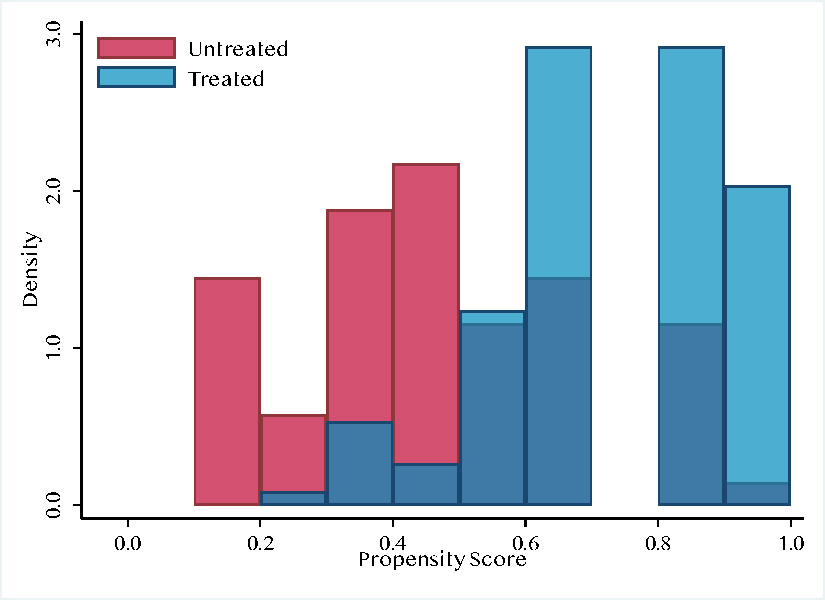
\includegraphics[width=\textwidth]{Figures/commonSupp.pdf}
         \caption{Probit}
     \end{subfigure}
     \begin{subfigure}[b]{0.47\textwidth}
         \centering
         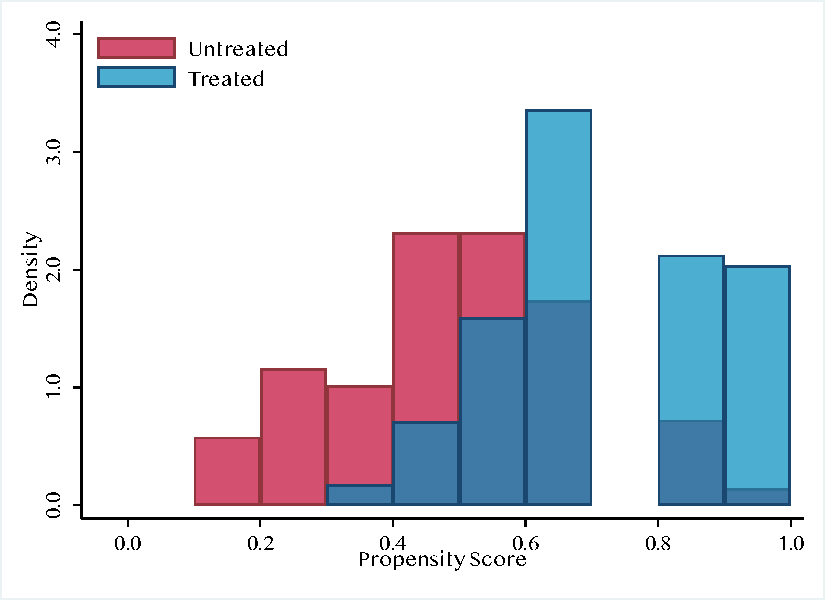
\includegraphics[width=\textwidth]{Figures/commonSuppLin.pdf}
         \caption{Linear Regression}
     \end{subfigure}
    \end{center}
    \vspace{-10pt}
    \scriptsize{}
\end{figure}
\FloatBarrier
Thus, for the analysis, the method of estimating the proensity score will matter. If done with the probit, the linearity should only consider data with $p\geq0.2$. If using the linear estimate, then the data that can be used for the analysis requires $p\geq 0.3.$. Next in Figure \ref{fig:linTest} we present the object described in equation \eqref{eq:func}. 
\begin{figure}[htb]
    \centering
    \caption{\sc Linear Test}
    \label{fig:linTest}
    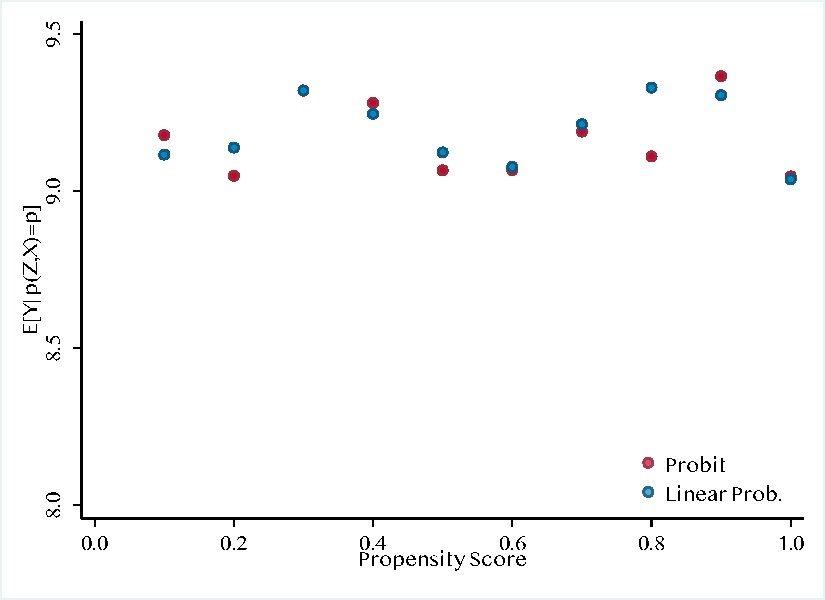
\includegraphics[width=0.48\textwidth]{Figures/Linear_Test.pdf}
\end{figure}
Upon inspection, it is clear that there are some non-linearities and thus we can not discard the possibility of sorting based on unobservables. A more formal test could be performed following \citet{Chen1999}. 

% Bibliography
\FloatBarrier
\newpage
\bibliographystyle{apacite}
\bibliography{Sections-Doc/references.bib}

\end{document}
